%%%%%%%%%%%%%%%%
\section{Control Approach}

\begin{frame}{Control Approach}{}
    \begin{figure}[H]
        \centering
        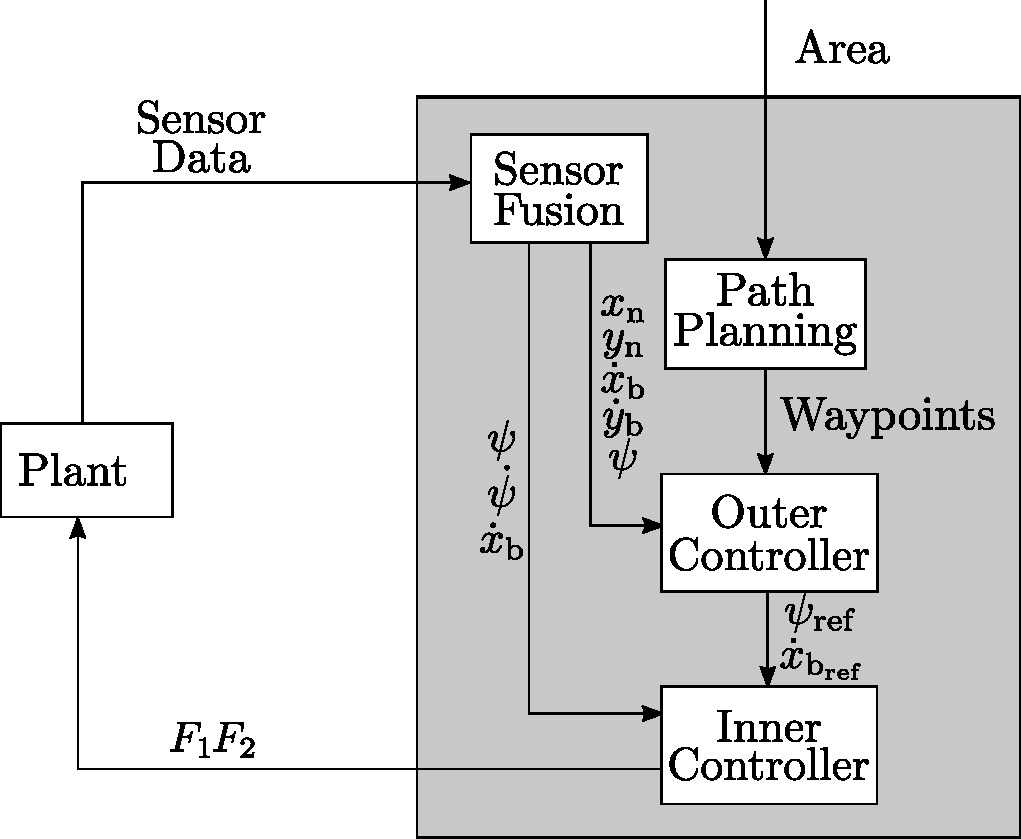
\includegraphics[width=.6\linewidth]{figures/controllerDiagram2}
    \end{figure}
\end{frame}

%%%%%%%%%%%%%%%%
\section{Sensor Fusion}

\begin{frame}{Sensor Fusion}{Structure}
	\begin{itemize}

		\item Fuses GPS and IMU data
		\item Achieved using a Kalman Filter
		\item Sensor Fusion Contains
			\begin{itemize}
		\item Attitude 
		\item Position 
			\end{itemize}
	\end{itemize}

\end{frame}
\begin{frame}{Sensor Fusion}{Signal Model}
	\begin{flalign}
	    \hat{\vec{x}}(k+1) &= \vec{A}\hat{\vec{x}}(k) + \vec{B} \vec{u}(k) + \vec{w}(k)  \nonumber \\
        \vec{y}(k) &= \vec{C} \hat{\vec{x}}(k) + \vec{v}(k)  \nonumber
	\end{flalign}

	\begin{itemize}
		\item w(k) and v(k) are assumed white Gaussian
	\end{itemize}




\end{frame}

\begin{frame}{Sensor Fusion}{Signal Model - State Extension}

States are extended to: 
\begin{itemize}
    \item Attitude: 
    \begin{flalign}
        \hat{\vec{x}}_\mathrm{att} &= 
        \begin{bmatrix}
        \phi & \theta & \psi & \dot{\phi} & \dot{\theta} & \dot{\psi} & \ddot{\phi} & \ddot{\theta} & \ddot{\psi}
        \end{bmatrix}^\mathrm{T}  \nonumber
    \end{flalign}
    \begin{flalign}
        \vec{y}_\mathrm{att} =
        \begin{bmatrix}
        \phi_\mathrm{acc} & \theta_\mathrm{acc} & \psi_\mathrm{mag} & \dot{\phi}_\mathrm{gyro} & \dot{\theta}_\mathrm{gyro} & \dot{\psi}_\mathrm{gyro}
        \end{bmatrix}^\mathrm{T} \nonumber
    \end{flalign}
	\item Position:
\begin{flalign}
        \hat{\vec{x}}_\mathrm{pos} &=
        \begin{bmatrix}
        x_\mathrm{n} & y_\mathrm{n} & \dot{x}_\mathrm{b} & \dot{y}_\mathrm{b} & \ddot{x}_\mathrm{b} & \ddot{y}_\mathrm{b}
        \end{bmatrix}^\mathrm{T} \nonumber
    \end{flalign}
    \begin{flalign}
        \vec{y}_\mathrm{pos} &=
        \begin{bmatrix}
        x_\mathrm{n,GPS} & y_\mathrm{n,GPS} & \ddot{x}_\mathrm{b,acc} & \ddot{y}_\mathrm{b,acc}
        \end{bmatrix}^\mathrm{T} \nonumber
    \end{flalign}
    \end{itemize}
\end{frame}


\begin{frame}{Sensor Fusion}{Kalman Filter}

	\begin{itemize}
		\item Step 0: Initialization
\begin{flalign}
	\hat{\vec{x}}_\mathrm{att}(0|0) &= \vec{0}_\mathrm{6x1} \ ,\\
	\vec{P}_\mathrm{att}(0|0) &= \vec{Q}_\mathrm{att}\ .
\end{flalign}
		\item Step 1: Prediction:
		\item Step 2: Update:
    	\end{itemize}
\end{frame}


\begin{frame}{Sensor Fusion}{Kalman Filter}

	\begin{itemize}
		\item Step 0: Initialization
		\item Step 1: Prediction:
    \begin{flalign}
        \hat{\vec{x}}(k+1|k) &= \vec{A} \hat{\vec{x}}(k|k) + \vec{B} \vec{u}(k) \nonumber\\
        \vec{P}(k+1|k) &= \vec{A} \vec{P}(k|k) \vec{A}^\mathrm{T} + \vec{Q} \nonumber
    \end{flalign}
	 	\item Step 2: Update:
    \begin{flalign}
        \hat{\vec{x}}(k+1|k+1) &= \hat{\vec{x}}(k+1|k) + \vec{K}(k+1) \left[ \vec{y}(k+1) - \vec{C}  \hat{\vec{x}}(k+1|k) \right] \nonumber\\
        \vec{P}(k+1|k+1) &= \left[ \vec{I} - \vec{K}(k+1) \vec{C}^\mathrm{T} \right] \vec{P}(k+1|k)\nonumber\\
	\vec{K}(k+1) &= \vec{P}(k+1|k) \vec{C}^\mathrm{T} \left[\vec{C} \vec{P}(k+1|k) \vec{C}^\mathrm{T} + \vec{R} \right]^{-1}\nonumber 
\end{flalign}
	\end{itemize}
	

\end{frame}

\begin{frame}{Sensor Fusion}{Attitude Kalman Filter}
    \begin{figure}[H]
        \centering
        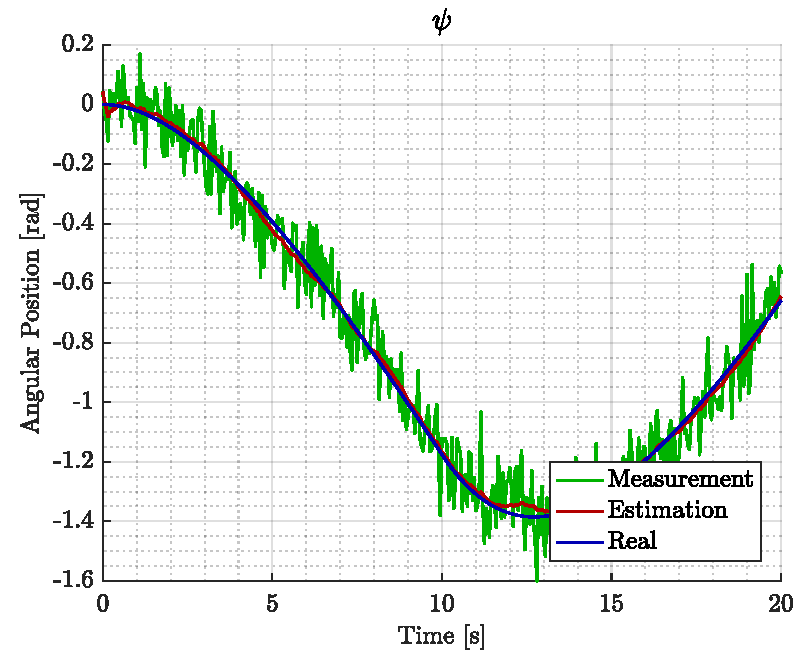
\includegraphics[width=0.6\linewidth]{figures/sim_yaw}
    \end{figure}
\end{frame}

\begin{frame}{Sensor Fusion}{Position Kalman Filter}
    \begin{minipage}{0.45\linewidth}
        \begin{figure}[H]
            \centering
            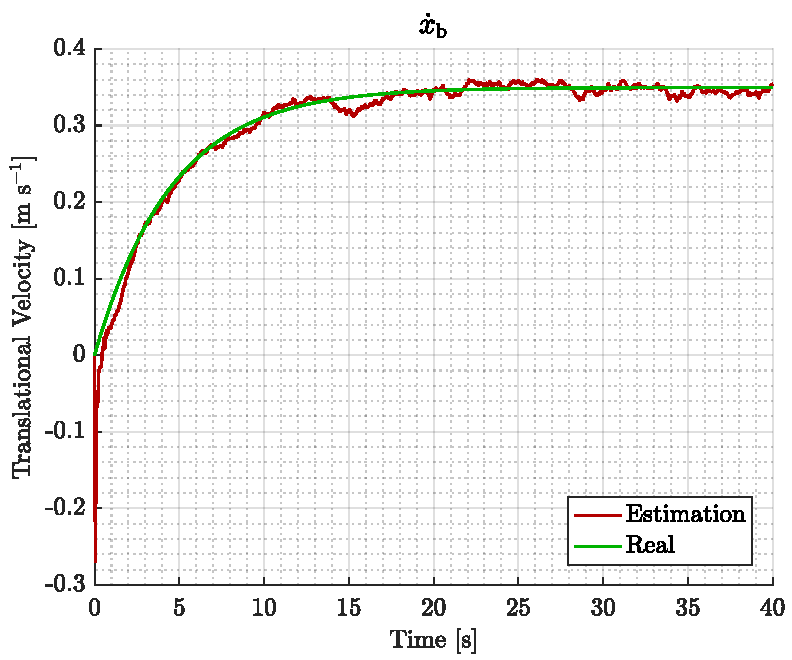
\includegraphics[width=1\linewidth]{figures/sim_xbdot}
        \end{figure}        
    \end{minipage}\hfill      
    \begin{minipage}{0.45\linewidth}
        \begin{figure}[H]
            \centering
            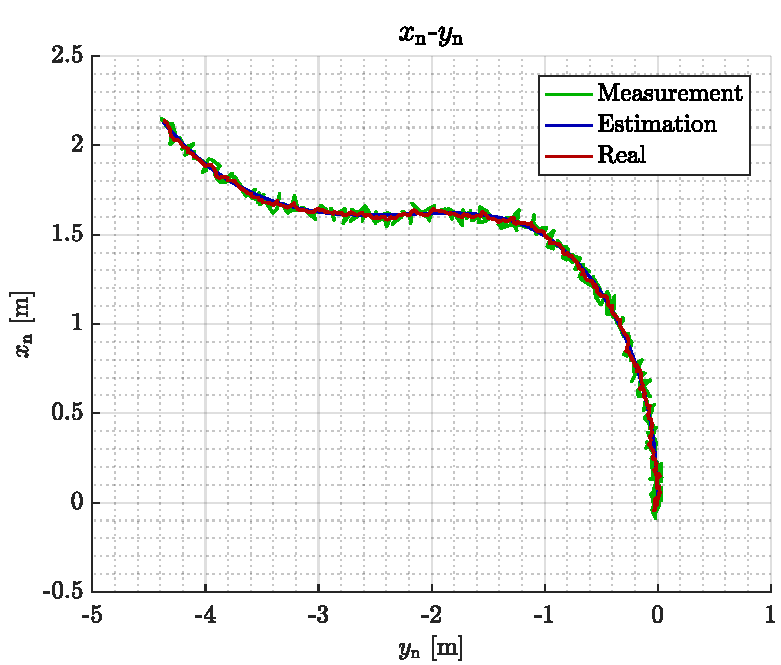
\includegraphics[width=1\linewidth]{figures/sim_xnyn}
        \end{figure}                
    \end{minipage}\hfill \\
\end{frame}

